\clearpage

\section{Month 3 - July}

\subsection{GEMMs (General Matrix Multiplications)}

General Matrix Multiplication (GEMM) is defined as the operation $C = AB + C$, with $A$ and $B$ as matrix inputs, and $C$ as a pre-existing matrix which is overwritten by the output.

\subsubsection{Math And Memory Bounds}


Matrix $A$ is an $M \times K$ matrix, meaning that it has $M$ rows and $K$ columns. Similarly, $B$ and $C$ are $K \times N$ and $M \times N$ matrices, respectively. The product of $A$ and $B$ has $M \times N$ values, each of which is a dot-product of $K$-element vectors.

Thus, a total of $M \times N \times K$ fused multiply-adds (FMAs) are needed to compute the product. Each FMA is 2 operations, a multiply and an add, so a total of $2 \times M \times N \times K$ FLOPS are required.


\begin{equation}
\text{Arithmetic Intensity} = \frac{\text{number of FLOPS}}{\text{number of byte accesses}} = \frac{2 \times (M \times N \times K)}{2 \times (M \times K + N \times K + M \times N)}
\end{equation}


For example, consider a $M \times N \times K = 5000 \times 5000 \times 5000$ GEMM. The arithmetic intensity can be calculated as:

\begin{equation}
\text{Arithmetic Intensity} = \frac{2 \times 5000 \times 5000 \times 5000}{2 \times (5000 \times 5000 + 5000 \times 5000 + 5000 \times 5000)} = 1666.67
\end{equation}

\textit{Bytes per FLOP (B/F) is a measurement of memory intensity per compute work or the amount of bytes required to be transferred between the execution unit and the off-chip memory relative to the number of floating-point operations required for a particular task.}

The calculated arithmetic intensity can be compared with the FLOPS:byte ratio to determine if the operation is memory or math limited. For example, the NVIDIA V100 GPU, the FLOPS:byte ratio is 138.9 (I couldn't find info for regular CPUs and GPUs as my Ryzen 5600X and my RTX 3070)

In our case, the arithmetic intensity for a $M \times N \times K = 5000 \times 5000 \times 5000$ GEMM is approximately 1666.67 FLOPS/B. This value is higher than the FLOPS:byte ratio of the NVIDIA V100 GPU. Therefore, this operation would be math limited, meaning the speed of the operation is constrained by the speed at which the GPU can perform calculations rather than the speed at which it can access memory.

If we were to decrease the size of the GEMM such that the resulting arithmetic intensity is lower than the FLOPS:byte ratio of the GPU, then the operation would become memory limited. In a memory limited operation, the speed of the operation is constrained by the speed at which the GPU can access memory rather than the speed at which it can perform calculations.

In particular, it follows from this analysis that matrix-vector products (general matrix-vector product or GEMV), where either $M=1$ or $N=1$, are always memory limited; their arithmetic intensity is less than 1.

Our goal is to determine the FLOPS:byte ratio for our various devices, including different types of CPUs and GPUs. This ratio is a key performance characteristic that can help us understand the balance between computational power and memory bandwidth in a given device. By understanding the FLOPS:byte ratio of our devices, we can make informed decisions about how to best utilize our computational resources.

\subsubsection{A Layered Approach to GEMM}
In the general case, GEMM can be systematically decomposed into multiple calls to special cases. These special cases include GEPP, GEMP, and GEPM operations. Each of these operations can be further decomposed into multiple calls to GEBP, GEPB, or GEPDOT kernels.

The idea is that if these three lowest level kernels attain high performance, then the other cases of GEMM will also perform well. This is illustrated in Fig. 5, which shows the path through the decomposition process that always takes the top branch.

By understanding this layered approach to GEMM, we can gain insights into the performance characteristics of different types of matrix multiplication operations and how they relate to each other.

\begin{figure}[H]
\centering
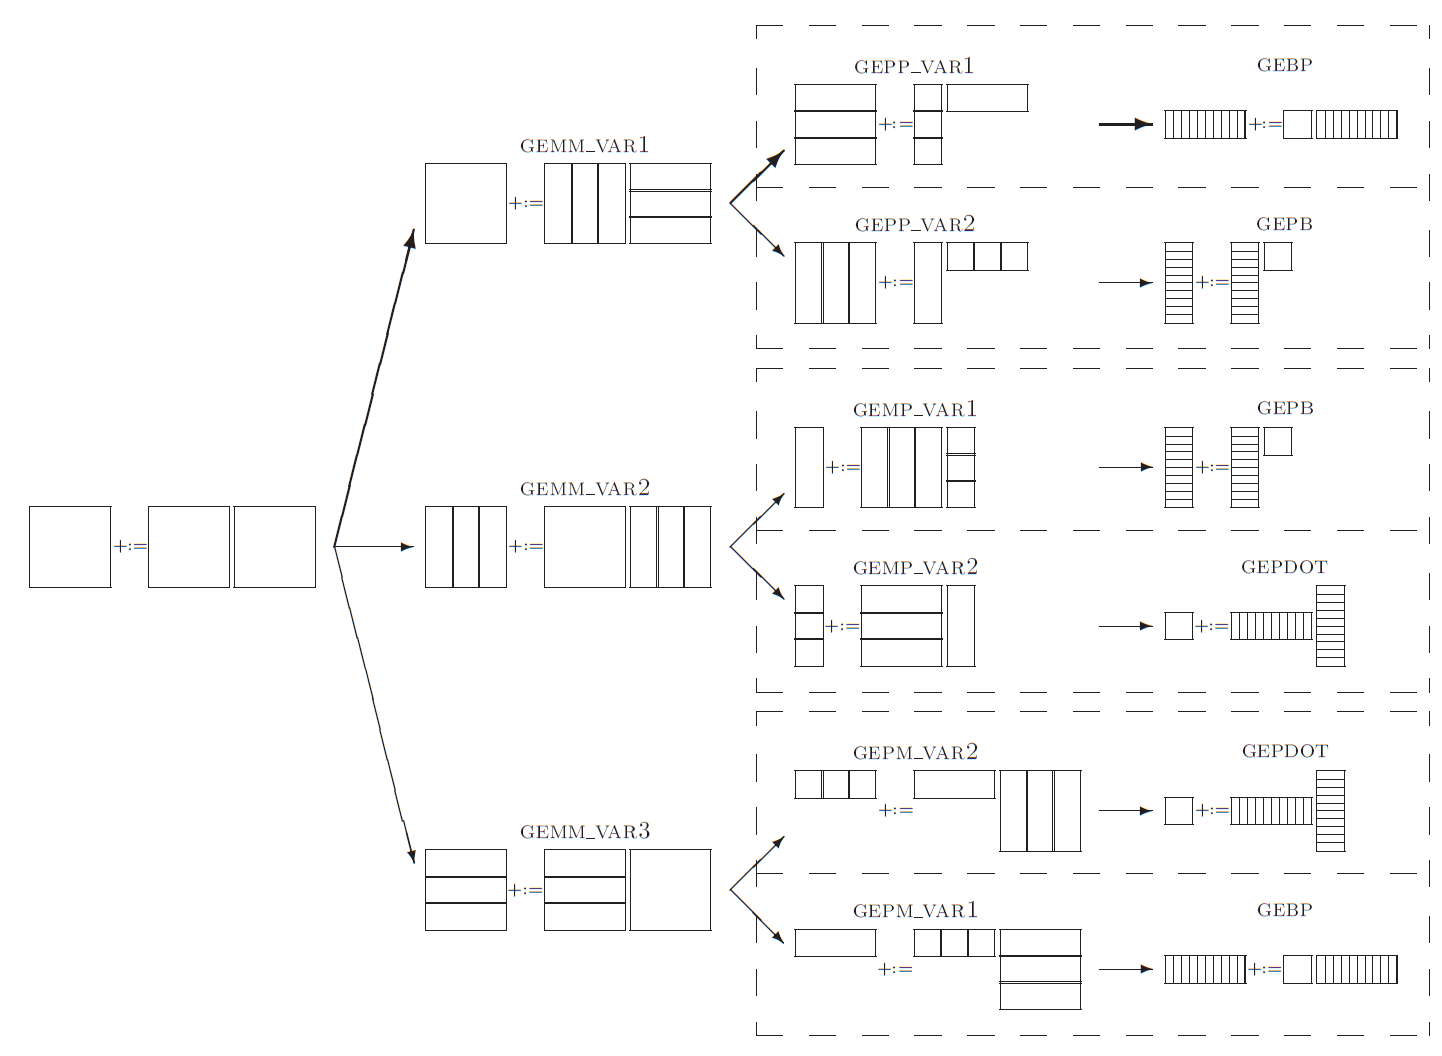
\includegraphics[width=130mm]{Figures/Imagenes/Special_cases_GEMM.png}
\caption{Layered approach to implementing gemm}
\end{figure}

\begin{itemize}
\item \textbf{GEPP (General Matrix-Panel Multiply):} This algorithm performs the multiplication of a general matrix by a panel (a subset of columns) of another matrix. It is useful when one wants to multiply a large matrix by a small submatrix of another matrix.

\item \textbf{GEMP (General Panel-Matrix Multiply):} This is the opposite case to GEPP. It performs the multiplication of a panel (a subset of columns) of a matrix by a general matrix. It is useful when one wants to multiply a small submatrix of a matrix by another large matrix.

\item \textbf{GEPM (General Panel-Panel Multiply):} This algorithm performs the multiplication of a panel (a subset of columns) of a matrix by another panel of another matrix. It is useful when one wants to multiply two small submatrices extracted from larger matrices.
\end{itemize}

As we said, each of these operations can be further decomposed into multiple calls to GEBP, GEPB, or GEPDOT kernels.

\begin{itemize}
\item \textbf{GEBP (General Panel-Block Multiply):} This algorithm performs the multiplication of a panel (a subset of columns) of a matrix by a block (a submatrix) of another matrix. It is useful when one wants to multiply a small submatrix of a matrix by a larger submatrix of another matrix.

\item \textbf{GEPB (General Panel-Block Multiply):} This algorithm performs the multiplication of a panel (a subset of columns) of a matrix by a block (a submatrix) of another matrix. It is useful when one wants to multiply a small submatrix of a matrix by a larger submatrix of another matrix.

\item \textbf{GEPDOT (General Panel-Dot Product):} This algorithm performs the dot product of a panel (a subset of columns) of a matrix with another panel of another matrix. It is useful when one wants to compute the dot product of two small submatrices extracted from larger matrices.
\end{itemize}

\subsubsection*{Cost of moving data between memory layers}
We now discuss techniques for the high-performance implementation of GEBP, GEPB, and GEPDOT. We do so by first analyzing the cost of moving data between memory layers with a naive model of the memory hierarchy. 

\begin{figure}[H]
\centering
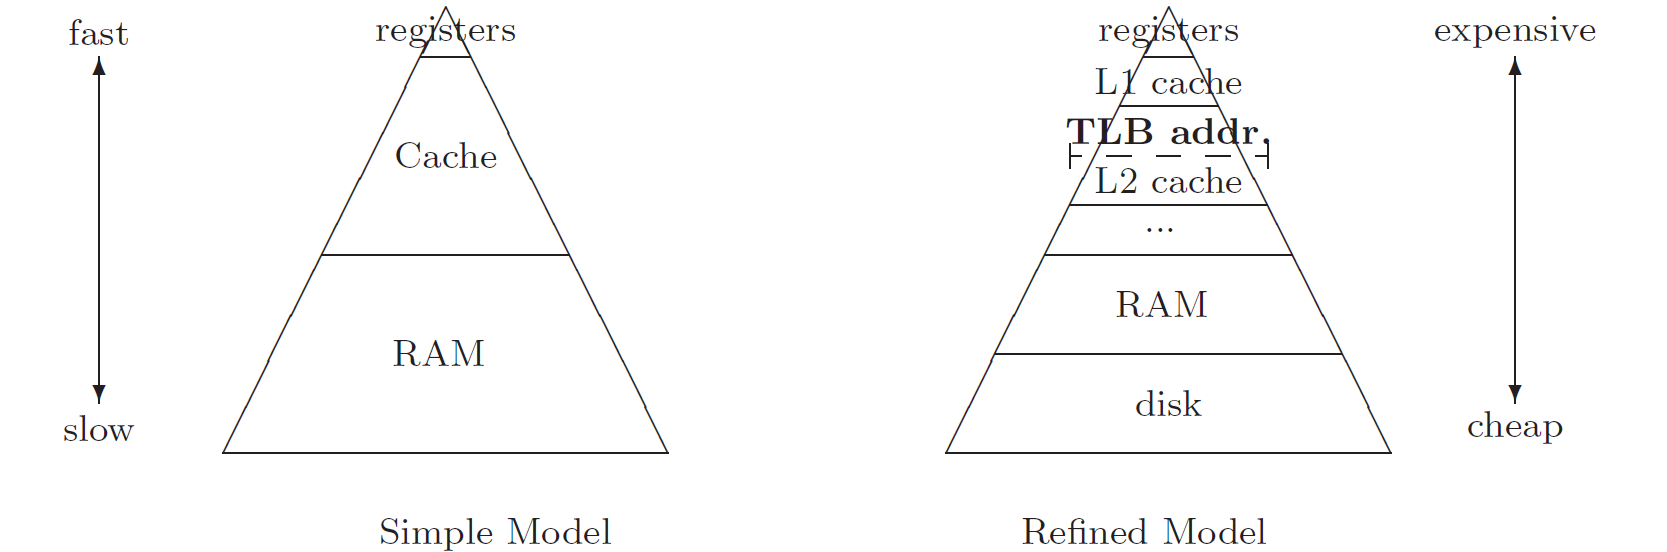
\includegraphics[width=90mm]{Figures/Imagenes/Memory_anatomy.png}
\caption{multi-level cache memory}
\end{figure}

We depict a very simple model of a multi-level cache memory. One layer of cache memory is inserted between the Random-Access Memory (RAM) and the registers. The top-level issues related to the high-performance implementation of GEBP, GEPB, and GEPDOT can be described using this simplified architecture.

\textit{TLB (Translation Lookaside Buffer) is a hardware cache used in processors to accelerate virtual address translation. It stores recently used virtual-to-physical address mappings, reducing the time required for address translation. TLB hits provide fast access to physical addresses, while TLB misses require accessing the page table in memory. TLBs are vital in modern processors for efficient virtual memory systems.}


\begin{figure}[H]
\centering
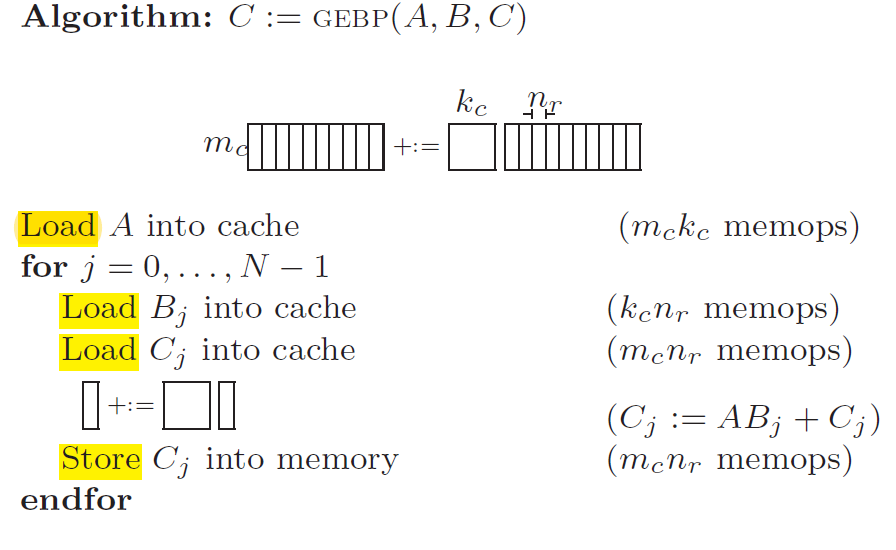
\includegraphics[width=110mm]{Figures/Imagenes/GEBP.png}
\caption{Basic implementation of GEBP}
\end{figure}


Assumption (a): The dimensions $mc$ and $kc$ are small enough so that matrix $A$ and $nr$ columns from each of $B$ and $C$ ($B_j$ and $C_j$, respectively) together fit in the cache.

Assumption (b): If $A$, $C_j$, and $B_j$ are in the cache, then the computation $C_j := AB_j + C_j$ can be performed at the peak rate of the CPU.

Assumption (c): If $A$ is in the cache, it remains there until it is no longer needed.


\clearpage

\subsection{Stack vs Heap}

\begin{itemize}
    \item \textbf{Heap:}
    \begin{enumerate}
        \item Available for the entire program with memory assigned dynamically.
        \item You can decide how much memory to allocate at runtime.
        \item Assigning and deallocating memory from the heap is relatively slow.
        \item In Fortran, global arrays and those allocated with ``allocate()'' are stored in the heap.
    \end{enumerate}

    \item \textbf{Stack:}
    \begin{enumerate}
        \item Has a more limited memory.
        \item Memory allocation and deallocation is very fast.
        \item Local arrays declared in a subroutine are stored in the stack.
        \item Each thread has its own stack.
    \end{enumerate}

    \item \textbf{Interaction between arrays and threads:}
    \begin{enumerate}
        \item All threads share the heap.
        \item If an array in the stack is created inside a parallel region, each thread will have its own copy.
        \item Synchronization is needed if multiple threads want to modify an array in the heap.
    \end{enumerate}

    \item \textbf{Recommendations:}
    \begin{enumerate}
        \item Allocate dynamic arrays only at a high level and infrequently.
        \item Use arrays in the stack for subroutine array temporaries.
        \item Understand the size of these arrays for a good estimation of the necessary stacksize.
    \end{enumerate}
\end{itemize}